% !TEX root = ./main.tex

\section{Numerics}
\label{sec:numerics}
\subsection{Flux Reconstruction Method}

What follows is an overview of the flux reconstruction (FR) framework. We start the discussion with the solution of the advection equation in one dimension using the FR approach to illustrate the peculiarities of the method. Then we proceed to describe the solution of the advection in two and three dimensions to show how the scheme works in triangular and tetrahedral elements. 
More details about FR and ESFR properties and derivations can be found in the articles and papers by Williams, Vincent, Castonguay, Jameson, and Huynh.

\subsubsection{Solution of the Advection Equation in One Dimension using the FR Approach}

Consider the one-dimensional conservation law
\begin{equation}
\label{eq:cons}
\frac{\partial u}{\partial t} + \frac{\partial f}{\partial x} = 0
\end{equation}

in domain $\Omega$, where $x$ is the spatial coordinate, $t$ is time, $u$ is a scalar function of $x$ and $t$, and $f$ is a scalar function of $u$. Note that letting $f = f(u,\frac{\partial u}{\partial x})$, Equation\ref{eq:cons} becomes a model of the Navier-Stokes equations.

Let us partition the domain $\Omega = [x_1,x_{N+1})$ into $N$ non-overlapping elements with 
interfaces at $x_1<x_2<...<x_{N+1}$. Then,
$$
\Omega = \bigcup^N_{n=1} \Omega_n
$$
and $\Omega_n = [x_n,x_{n+1})$ for $n = 1,...,N$.

To simplify the implementation, let us map each of the physical elements $\Omega_n$ to a standard 
element $\Omega_s=[-1,1)$ with the function $\Theta_n(\xi)$, where
$$
x = \Theta_n(\xi) = \l( \frac{1-\xi}{2} \r) x_n + \l(\frac{1+\xi}{2}\r) x_{n+1} 
$$

With this mapping, the evolution of $u$ within each $\Omega_n$ can be determined with the following 
transformed advection equation
$$
\frac{\partial \hat{u}}{\partial t} + \frac{\partial \hat{f}}{\partial \xi} = 0
$$
where
$$
\hat{u} = J_n u(\Theta_n(\xi),t) \text{ in } \Omega_n
$$
$$
\hat{f} = f(\Theta_n(\xi),t) \text{ in } \Omega_n
$$

Now, introduce polynomial approximations $\hat{u}^\delta, \hat{f}^\delta$ to 
the exact values $\hat{u},\hat{f}$, respectively. Using piecewise polynomials of degree $p$ as 
approximations, we can write
$$
\hat{u}^\delta = \sum_{i=1}^{N_s} \hat{u}_i^\delta l_i(\xi)
$$
$$
\hat{f}^\delta = \sum_{i=1}^{N_s} \hat{f}_i^\delta l_i(\xi)
$$
where $N_s$ is the number of solution points, $\hat{u}_i^\delta$ is the current value of the 
solution approximation function at the $i^\text{th}$ solution point in the reference element, 
$\hat{f}_i^\delta$ is the current value of the flux approximation function at the $i^\text{th}$ 
solution point in the reference element, $l_i$ is the Lagrange polynomial equal to $1$ at the 
$i^\text{th}$ solution point and $0$ in the others, and $\delta$ signals that the function is an 
approximation.

Note that the piecewise polynomials may not be continuous (or $c_0$) accross the interfaces. In the 
Flux Reconstruction approach, the flux used in the time advancement of the solution is made $c_0$ 
by introducing flux correction functions. To this end, in the general non-linear advection case, it 
is necessary to first make the solution $c_0$.

This can be done by finding interface values at each element and then correcting the 
solution. Let $\hat{u}_L^{\delta I}$ and $\hat{u}_R^{\delta I}$ be the interface values at left and right 
boundaries of each element, respectively. Then, select solution correction functions $g_L$ and 
$g_R$ such 
that
$$
g_L(-1) = 1 \; g_L(1) = 0
$$
$$
g_R(-1) = 0 \; g_R(1) = 1
$$
and let
$$
\hat{u}^c = \hat{u}^\delta + (\hat{u}^{\delta I}_L - \hat{u}^\delta_L) g_L + (\hat{u}^{\delta I}_R 
- \hat{u}^\delta_R) g_R
$$
where superscript $c$ denotes the function is corrected, and $\hat{u}^\delta_L$, $\hat{u}^\delta_R$ 
represent the solution approximation evaluated at the left and right boundaries.

We can proceed in a similar fashion to correct the flux to obtain
$$
\hat{f}^c = \hat{f}^\delta + (\hat{f}^{\delta I}_L - \hat{f}^\delta_L) h_L + (\hat{f}^{\delta I}_R 
- \hat{f}^\delta_R) h_R
$$
where $h_R$ and $h_L$ are right and left flux correction functions satisfying the same boundary 
conditions as $g_R$ and $g_L$, respectively.

The solution can then be advanced at each solution point. In semi-discrete form, this is
$$
\frac{d \hat{u}_i^\delta}{d t} = - \frac{\partial \hat{f}^c}{\partial \xi}(\xi_i)
$$

The FR scheme can be made stable by selecting special types of correction functions.

%The final paper, for completeness, will include a description of the Flux Reconstruction\cite{vincent2011new} approach and the reasoning behind using the Energy-Stable version. A thorough description of the steps taken in the calculation of the residual for the 3D NS Equations will be included.


\subsection{Unstructured Mesh Treatment}
Mention developments in squares (tensor products of linear scheme), triangles\cite{castonguay2012new,williams2013tri}, tetrahedra\cite{williams2013tet}, prisms (tensor product of linear with triangular schemes), and hexahedra (tensor products of linear scheme).

\subsection{Time Stepping and p-multigrid}
Explicit RK4 with ability to use multigrid\cite{fidkowski2005p} and dual time-stepping\cite{Jameson1991DualTime} for implicit time advancement.

%\subsection{Stabilization Techniques}

\subsection{Large Eddy Simulation Models}\label{lesmodels}
SGS Models: Smagorinsky\cite{smagorinsky1963}, WALE\cite{nicoud1999}, WALE-similarity\cite{lodato2009}, SVV\cite{karamanos2000}.
Filters: Vasilyev\cite{vasilyev1998,vasilyev2001}, discrete Gaussian\cite{lodato2012b}, Modal Vandermonde\cite{blackburn2003}.

In order to resolve all the scales of motion in a high Reynolds number turbulent flow, the computational mesh would have to be impractically fine.
A practical solution is to employ the Large Eddy Simulation (LES) formulation, which only resolves the larger scales of motion and thus allows for the use of coarser meshes.
The effect of the unresolved or subgrid-scale (SGS) dynamics on the solution is accounted for by an SGS model for the \emph{subgrid-scale stress} $\bar{\bar{\tau}}_{sgs}$, which is added to the viscous stress tensor $\bar{\bar{\tau}}$ given by (\ref{tau}):
%
\begin{equation}\label{tausgs}
\bar{\bar{\tau}} = \mu \left ( \nabla \vec{v} + {\nabla \vec{v}}^\mathsf{T}  - \frac{2}{3} \bar{\bar{I}} (\nabla \cdot \vec{v} ) \right ) + \bar{\bar{\tau}}_{sgs}.
\end{equation}
%
The standard Smagorinsky model is available in HiFiLES and is given by:
%
\begin{eqnarray}\label{smag}
\bar{\bar{\tau}}_{sgs} &&= 2 \rho \nu_t \bar{\bar{S^d}}, \\
\nu_t &&= C_S^2 \bigtriangleup^2 | \bar{\bar{S^d}} |,\\
\bar{\bar{S^d}} &&= \frac 1 2 \left (\nabla \vec v + (\nabla \vec v)^T - \frac 2 3 \bar{\bar{I}} (\nabla \cdot \vec{v} ) \right )\ ,
\end{eqnarray}
%
where the Smagorinsky coefficient $C_S = 0.1$ and the filter width $\bigtriangleup$ is a measure of the size of an element.
The quantity $\nu_t$ is the eddy viscosity.
In HiFiLES the filter width is given by (in 3D):
%
\begin{equation}
\bigtriangleup = \alpha (\text{vol})^{1/3},
\end{equation}
%
where $\alpha \geq 1$ is a user-defined scaling factor and vol is the element volume.
HiFiLES also includes the Wall-Adapting Local Eddy-Viscosity (WALE) model~\cite{nicoud1999} and the Similarity model~\cite{bardina1980}.
The Similarity model incorporates a filtering operator that locally smoothes the solution in order to extract small-scale information.
Several filters are available in HiFiLES: a discrete Gaussian filter, a high-order commuting Vasilyev-type filter and a modal Vandermonde-type filter.
For details of these operators, see Lodato, Castonguay and Jameson~\cite{lodato2012b} and Bull and Jameson~\cite{bull2013a}.
Also available is the option to combine the similarity model and either the Smagorinsky or WALE model into a mixed model.
The mixed WALE-similarity model, developed by Lodato et al.~\cite{lodato2009}, was used in simulations of the flow over a square cylinder (see Section \ref{sqcyl}).
Finally, a Spectral Vanishing Viscosity (SVV) model is available.
Instead of adding a model term, the SVV method applies a filter directly to the solution in order to damp high-order modes~\cite{karamanos2000}.

\subsection{Computing Architecture and Scalability}
%The final paper will include a description of how HiFiLES is designed for a multi-GPU environment. Studies performed without filtering or SGS modeling in \cite{castonguay2011}. 

The HiFiLES code has been designed to work on multi-CPU as well as multi-CPU-GPU platforms. The Flux Reconstruction method in its current form with explicit time-stepping has a great potential for parallelization. Since the solution points are not explicitly shared between elements, most of the computations are element-local enabling an efficient use of shared memory on GPUs. Also, several computations are independent for each solution point and the highly parallelizable nature of GPUs becomes very useful. A detailed description of the paralleization of the FR method, along with scalability and performance analysis has been performed in \cite{castonguay2011}.

\subsection{Shock capturing and Stabilization Models}


Currently, we have adapted Persson and Peraire's method \cite{Persson06} for shock detection and capturing. The method works well for inviscid flow cases and compressible flows upto a Mach number of 2 have been tried and tested. However the method requires fine-tuning of parameters for each problem and we are currently working on a new method which is more robust. Persson and Peraire have used this shock capturing tool as a stabilization method as well in their turbulence calculations and we plan to test this and present results for inviscid and viscous cases in the final draft. Here we show a few inviscid results for the case of M = 1.6 where we illustrate the ability to detect shocks and add dissipation in a local manner in the form of artificial viscosity in order to capture the shock in a fine manner and avoid the loss of accuracy away from the shock.    

\begin{figure}[h] \tt
\centering
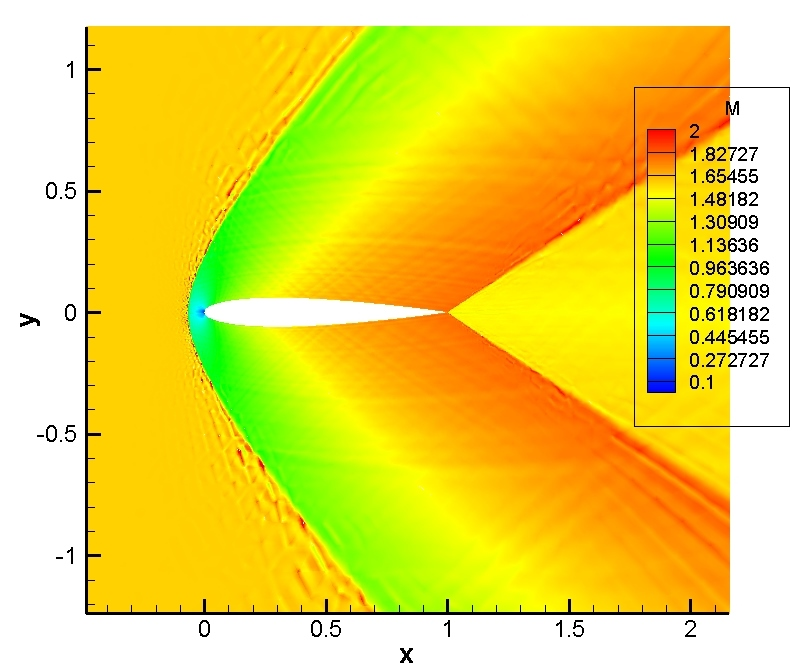
\includegraphics[angle=0, scale = 0.55]{./figures/M1pt6order3-inv-720ktime-mach.jpg} \\
\caption{Mach contours for inviscid flow over Naca0012 at M = 1.6 and AoA = $0^{\circ} $}
\label{fig:inv_mach}
\end{figure}

\begin{figure}
\centering
\begin{minipage}[t]{.5\textwidth}
  \centering
  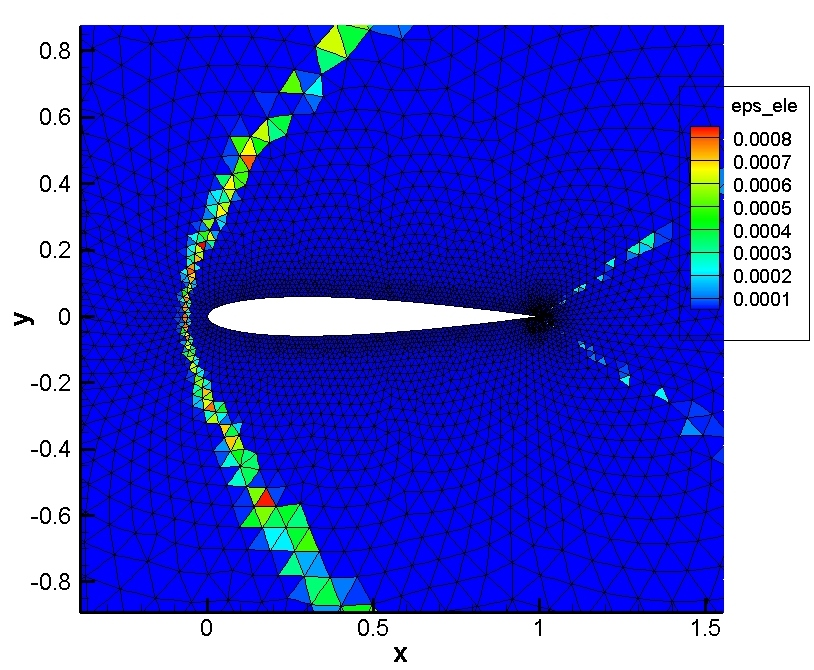
\includegraphics[width=.85\linewidth]{./figures/M1pt6-inv-av-ele-mesh}
  \captionof{figure}{Element-wise AV co-efficients (case 1)}
  \label{fig:AV-ele}
\end{minipage}%
\begin{minipage}[t]{.5\textwidth}
  \centering
  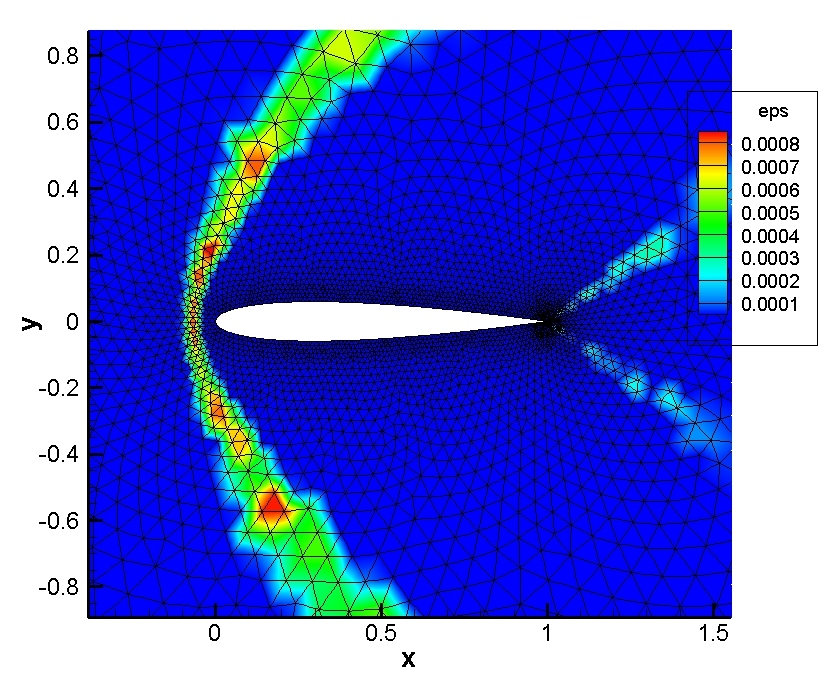
\includegraphics[width=.85\linewidth]{./figures/M1pt6-inv-av-mesh}
  \captionof{figure}{AV co-efficients with continuity enforcement}
  \label{fig:AV-cont}
\end{minipage}
\end{figure} 

